\documentclass[../main.tex]{subfiles}
\begin{document}

\theoremstyle{definition}

\chapter{Linear Algebraic Equations
and Matrices}
\label{cha8:cha8}
\begin{center}
\Large{\textbf{CHAPTER OBJECTIVES}}
\end{center}

The primary objective of this chapter is to acquaint you with linear algebraic equations and their relationship to matrices and matrix algebra. Specific objectives and topics covered are
\begin{itemize}
\item Understanding matrix notation.
\item Being able to identify the following types of matrices: identity, diagonal, symmetric, triangular, and tridiagonal.
\item Knowing how to perform matrix multiplication and being able to assess when it is feasible.
\item Knowing how to represent a system of linear algebraic equations in matrix form.
\item Knowing how to solve linear algebraic equations with left division and matrix inversion in MATLAB.
\end{itemize}
\bigskip

\Large{YOU'VE GOT A PROBLEM}
\normalsize
\bigskip

Suppose that three jumpers are connected by bungee cords. Figure 8.1 $a$ shows them being held in place vertically so that each cord is fully extended but unstretched. We can define three distances, $x_{1}, x_{2}$, and $x_{3}$, as measured downward from each of their unstretched positions. After they are released, gravity takes hold and the jumpers will eventually come to the equilibrium positions shown in Fig. 8.1b.

Suppose that you are asked to compute the displacement of each of the jumpers. If we assume that each cord behaves as a linear spring and follows Hooke's law, free-body diagrams can be developed for each jumper as depicted in Fig. 8.2.
\newpage

\begin{multicols}{2}

\begin{figure}[H]
	\centering
	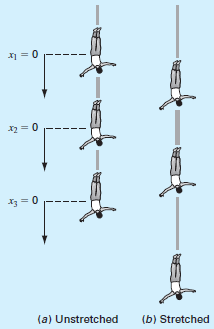
\includegraphics[width=0.7\linewidth]{fig_8_1}
	\caption{\textsf{Three individuals connected by bungee cords.}}
	\label{fig:fig_8_1}
\end{figure}

\begin{figure}[H]
	\centering
	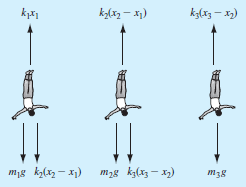
\includegraphics[width=1\linewidth]{fig_8_2}
	\caption{\textsf{Free-body diagrams.}}
	\label{fig:fig_8_2}
\end{figure}

\end{multicols}

Using Newton's second law, force balances can be written for each jumper:
$$
\begin{aligned}
&m_{1} \frac{d^{2} x_{1}}{d t^{2}}=m_{1} g+k_{2}\left(x_{2}-x_{1}\right)-k_{1} x_{1} \\
&m_{2} \frac{d^{2} x_{2}}{d t^{2}}=m_{2} g+k_{3}\left(x_{3}-x_{2}\right)+k_{2}\left(x_{1}-x_{2}\right) \\
&m_{3} \frac{d^{2} x_{3}}{d t^{2}}=m_{3} g+k_{3}\left(x_{2}-x_{3}\right)
\end{aligned}
$$ \hfill{(8.1)}

where $m_{i}=$ the mass of jumper $i(\mathrm{~kg}), t=$ time $(\mathrm{s}), k_{j}=$ the spring constant for cord $j(\mathrm{~N} / \mathrm{m}), x_{i}=$ the displacement of jumper $i$ measured downward from the equilibrium position $(\mathrm{m})$, and $g=$ gravitational acceleration $\left(9.81 \mathrm{~m} / \mathrm{s}^{2}\right)$. Because we are interested in the steady-state solution, the second derivatives can be set to zero. Collecting terms gives
$$
\begin{aligned}
\left(k_{1}+k_{2}\right) x_{1}-k_{2} x_{2} &=m_{1} g \\
-k_{2} x_{1}+\left(k_{2}+k_{3}\right) x_{2}-k_{3} x_{3} &=m_{2} g \\
-k_{3} x_{2}+k_{3} x_{3} &=m_{3} g
\end{aligned}
$$ \hfill{(8.2)}

Thus, the problem reduces to solving a system of three simultaneous equations for the three unknown displacements. Because we have used a linear law for the cords, these equations are linear algebraic equations. Chapters 8 through 12 will introduce you to how MATLAB is used to solve such systems of equations.

\bigskip
\section{MATRIX ALGEBRA OVERVIEW}
\label{sec:sec_8_1}

Knowledge of matrices is essential for understanding the solution of linear algebraic equations. The following sections outline how matrices provide a concise way to represent and manipulate linear algebraic equations.

\subsection{Matrix Notation}

\noindent A matrix consists of a rectangular array of elements represented by a single symbol. As depicted in Fig. $8.3,[A]$ is the shorthand notation for the matrix and $a_{i j}$ designates an individual element of the matrix.

A horizontal set of elements is called a row and a vertical set is called a column. The first subscript $i$ always designates the number of the row in which the element lies. The second subscript $j$ designates the column. For example, element $a_{23}$ is in row 2 and column 3 .

The matrix in Fig. $8.3$ has $m$ rows and $n$ columns and is said to have a dimension of $m$ by $n$ (or $m \times n$ ). It is referred to as an $m$ by $n$ matrix.

Matrices with row dimension $m=1$, such as
$$
[b]=\left[\begin{array}{llll}
b_{1} & b_{2} & \cdots & b_{n}
\end{array}\right]
$$
are called row vectors. Note that for simplicity, the first subscript of each element is dropped. Also, it should be mentioned that there are times when it is desirable to employ a special shorthand notation to distinguish a row matrix from other types of matrices. One way to accomplish this is to employ special open-topped brackets, as in $\lfloor b\rfloor.$

Matrices with column dimension $n=1$, such as
$$
[c]=\left[\begin{array}{c}
c_{1} \\
c_{2} \\
\vdots \\
c_{m}
\end{array}\right]
$$

\begin{figure}[H]
	\centering
	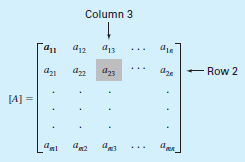
\includegraphics[width=0.4\linewidth]{fig_8_3}
	\caption{\textsf{A matrix.}}
	\label{fig:fig_8_3}
\end{figure}

\noindent are referred to as column vectors. For simplicity, the second subscript is dropped. As with the row vector, there are occasions when it is desirable to employ a special shorthand notation to distinguish a column matrix from other types of matrices. One way to accomplish this is to employ special brackets, as in $\{c\}$.

Matrices where $m=n$ are called square matrices. For example, a $3 \times 3$ matrix is
$$
[A]=\left[\begin{array}{lll}
a_{11} & a_{12} & a_{13} \\
a_{21} & a_{22} & a_{23} \\
a_{31} & a_{32} & a_{33}
\end{array}\right]
$$
The diagonal consisting of the elements $a_{11}, a_{22}$, and $a_{33}$ is termed the principal or main diagonal of the matrix.

Square matrices are particularly important when solving sets of simultaneous linear equations. For such systems, the number of equations (corresponding to rows) and the number of unknowns (corresponding to columns) must be equal for a unique solution to be possible. Consequently, square matrices of coefficients are encountered when dealing with such systems.

There are a number of special forms of square matrices that are important and should be noted:

A symmetric matrix is one where the rows equal the columns - that is, $a_{i j}=a_{j i}$ for all $i$ 's and $j$ 's. For example,
$$
[A]=\left[\begin{array}{lll}
5 & 1 & 2 \\
1 & 3 & 7 \\
2 & 7 & 8
\end{array}\right]
$$
is a $3 \times 3$ symmetric matrix.

A diagonal matrix is a square matrix where all elements off the main diagonal are equal to zero, as in
$$
[A]=\left[\begin{array}{lll}
a_{11} & & \\
& a_{22} & \\
& & a_{33}
\end{array}\right]
$$
Note that where large blocks of elements are zero, they are left blank.

An identity matrix is a diagonal matrix where all elements on the main diagonal are equal to 1 , as in
$$
[I]=\left[\begin{array}{lll}
1 & & \\
& 1 & \\
& & 1
\end{array}\right]
$$
The identity matrix has properties similar to unity. That is,
$$
[A][I]=[I][A]=[A]
$$
An upper triangular matrix is one where all the elements below the main diagonal are zero, as in
$$
[A]=\left[\begin{array}{lll}
a_{11} & a_{12} & a_{13} \\
& a_{22} & a_{23} \\
& & a_{33}
\end{array}\right]
$$

A lower triangular matrix is one where all elements above the main diagonal are zero, as in
$$
[A]=\left[\begin{array}{lll}
a_{11} & & \\
a_{21} & a_{22} & \\
a_{31} & a_{32} & a_{33}
\end{array}\right]
$$

A banded matrix has all elements equal to zero, with the exception of a band centered on the main diagonal:
$$
[A]=\left[\begin{array}{llll}
a_{11} & a_{12} & & \\
a_{21} & a_{22} & a_{23} & \\
& a_{32} & a_{33} & a_{34} \\
& & a_{43} & a_{44}
\end{array}\right]
$$
The preceding matrix has a bandwidth of 3 and is given a special name-the tridiagonal matrix.

\subsection{Matrix Operating Rules}

Now that we have specified what we mean by a matrix, we can define some operating rules that govern its use. Two $m$ by $n$ matrices are equal if, and only if, every element in the first is equal to every element in the second-that is, $[A]=[B]$ if $a_{i j}=b_{i j}$ for all $i$ and $j$.

Addition of two matrices, say, $[A]$ and $[B]$, is accomplished by adding corresponding terms in each matrix. The elements of the resulting matrix $[C]$ are computed as
$$
c_{i j}=a_{i j}+b_{i j}
$$
for $i=1,2, \ldots, m$ and $j=1,2, \ldots, n$. Similarly, the subtraction of two matrices, say, $[E]$ minus $[F]$, is obtained by subtracting corresponding terms, as in
$$
d_{i j}=e_{i j}-f_{i j}
$$
for $i=1,2, \ldots, m$ and $j=1,2, \ldots, n$. It follows directly from the preceding definitions that addition and subtraction can be performed only between matrices having the same dimensions.
Both addition and subtraction are commutative:
$$
[A]+[B]=[B]+[A]
$$
and associative:
$$
([A]+[B])+[C]=[A]+([B]+[C])
$$
The multiplication of a matrix $[A]$ by a scalar $g$ is obtained by multiplying every element of $[A]$ by $g$. For example, for a $3 \times 3$ matrix:
$$
[D]=g[A]=\left[\begin{array}{lll}
g a_{11} & g a_{12} & g a_{13} \\
g a_{21} & g a_{22} & g a_{23} \\
g a_{31} & g a_{32} & g a_{33}
\end{array}\right]
$$

\begin{multicols}{2}

    \begin{figure}[H]
        \centering
        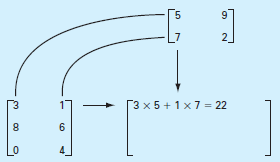
\includegraphics[width=0.7\linewidth]{fig_8_4}
        \caption{\textsf{Visual depiction of how the rows and columns line up in
        matrix multiplication.}}
        \label{fig:fig_8_4}
    \end{figure}
    
    \begin{figure}[H]
        \centering
        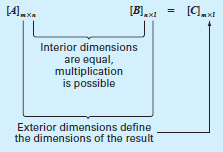
\includegraphics[width=0.7\linewidth]{fig_8_5}
        \caption{\textsf{Matrix multiplication can be performed only if
        the inner dimensions are equal.}}
        \label{fig:fig_8_5}
    \end{figure}
    
\end{multicols}


The product of two matrices is represented as $[C]=[A][B]$, where the elements of $[C]$ are defined as
\\

$c_{i j}=\sum_{k=1}^{n} a_{i k} b_{k j}$\hfill{(8.4)}\\


\noindent where $n=$ the column dimension of $[A]$ and the row dimension of $[B]$. That is, the $c_{i j}$ element is obtained by adding the product of individual elements from the $i$ th row of the first matrix, in this case $[A]$, by the $j$ th column of the second matrix $[B]$. Figure $8.4$ depicts how the rows and columns line up in matrix multiplication.

According to this definition, matrix multiplication can be performed only if the first matrix has as many columns as the number of rows in the second matrix. Thus, if $[A]$ is an $m$ by $n$ matrix, $[B]$ could be an $n$ by $l$ matrix. For this case, the resulting $[C]$ matrix would have the dimension of $m$ by $l$. However, if $[B]$ were an $m$ by $l$ matrix, the multiplication could not be performed. Figure $8.5$ provides an easy way to check whether two matrices can be multiplied.

If the dimensions of the matrices are suitable, matrix multiplication is associative:
$$
([A][B])[C]=[A]([B][C])
$$
and distributive:
$$
[A]([B]+[C])=[A][B]+[A][C]
$$
or
$$
([A]+[B])[C]=[A][C]+[B][C]
$$
However, multiplication is not generally commutative:
$$
[A][B] \neq[B][A]
$$
That is, the order of matrix multiplication is important.

Although multiplication is possible, matrix division is not a defined operation. However, if a matrix $[A]$ is square and nonsingular, there is another matrix $[A]^{-1}$, called the inverse of $[A]$, for which
$$
[A][A]^{-1}=[A]^{-1}[A]=[I]
$$
Thus, the multiplication of a matrix by the inverse is analogous to division, in the sense that a number divided by itself is equal to 1 . That is, multiplication of a matrix by its inverse leads to the identity matrix.
The inverse of a $2 \times 2$ matrix can be represented simply by
$$
[A]^{-1}=\frac{1}{a_{11} a_{22}-a_{12} a_{21}}\left[\begin{array}{cc}
a_{22} & -a_{12} \\
-a_{21} & a_{11}
\end{array}\right]
$$
Similar formulas for higher-dimensional matrices are much more involved. Chapter 11 will deal with techniques for using numerical methods and the computer to calculate the inverse for such systems.

The transpose of a matrix involves transforming its rows into columns and its columns into rows. For example, for the $3 \times 3$ matrix:
$$
[A]=\left[\begin{array}{lll}
a_{11} & a_{12} & a_{13} \\
a_{21} & a_{22} & a_{23} \\
a_{31} & a_{32} & a_{33}
\end{array}\right]
$$
the transpose, designated $[A]^{T}$, is defined as
$$
[A]^{T}=\left[\begin{array}{lll}
a_{11} & a_{21} & a_{31} \\
a_{12} & a_{22} & a_{32} \\
a_{13} & a_{23} & a_{33}
\end{array}\right]
$$
In other words, the element $a_{i j}$ of the transpose is equal to the $a_{j i}$ element of the original matrix.

The transpose has a variety of functions in matrix algebra. One simple advantage is that it allows a column vector to be written as a row, and vice versa. For example, if
$$
\{c\}=\left\{\begin{array}{l}
c_{1} \\
c_{1} \\
c_{1}
\end{array}\right\}
$$
then
$$
\{c\}^{T}=\left[\begin{array}{lll}
c_{1} & c_{2} & c_{3}
\end{array}\right]
$$
In addition, the transpose has numerous mathematical applications.
A permutation matrix (also called a transposition matrix) is an identity matrix with rows and columns interchanged. For example, here is a permutation matrix that is constructed by switching the first and third rows and columns of a $3 \times 3$ identity matrix:
$$
[P]=\left[\begin{array}{lll}
0 & 0 & 1 \\
0 & 1 & 0 \\
1 & 0 & 0
\end{array}\right]
$$

Left multiplying a matrix $[A]$ by this matrix, as in $[P][A]$, will switch the corresponding rows of $[A]$. Right multiplying, as in $[A][P]$, will switch the corresponding columns. Here is an example of left multiplication:
$$
[P][A]=\left[\begin{array}{lll}
0 & 0 & 1 \\
0 & 1 & 0 \\
1 & 0 & 0
\end{array}\right]\left[\begin{array}{ccc}
2 & -7 & 4 \\
8 & 3 & -6 \\
5 & 1 & 9
\end{array}\right]=\left[\begin{array}{ccc}
5 & 1 & 9 \\
8 & 3 & -6 \\
2 & -7 & 4
\end{array}\right]
$$
The final matrix manipulation that will have utility in our discussion is augmentation. A matrix is augmented by the addition of a column (or columns) to the original matrix. For example, suppose we have a $3 \times 3$ matrix of coefficients. We might wish to augment this matrix $[A]$ with a $3 \times 3$ identity matrix to yield a $3 \times 6$ dimensional matrix:
$$
\left[\begin{array}{lll|lll}
a_{11} & a_{11} & a_{11} & 1 & 0 & 0 \\
a_{21} & a_{21} & a_{21} & 0 & 1 & 0 \\
a_{31} & a_{31} & a_{31} & 0 & 0 & 1
\end{array}\right]
$$
Such an expression has utility when we must perform a set of identical operations on the rows of two matrices. Thus, we can perform the operations on the single augmented matrix rather than on the two individual matrices.

\begin{example} MATLAB Matrix Manipulations\\

    \noindent\textbf{Problem Statement.}\quad The following example illustrates how a variety of matrix manipulations are implemented with MATLAB. It is best approached as a hands-on exercise on the computer.\\


    \noindent\textbf{Solution.}\quad Create a $3 \times 3$ matrix:\\

    \begin{lstlisting}[numbers=none,frame=none]
        >> A = [1 5 6;7 4 2;-3 6 7]
        A =
            1 5 6
            7 4 2
            -3 6 7
	\end{lstlisting}

    \noindent The transpose of $[A]$ can be obtained using the " operator:

    \begin{lstlisting}[numbers=none,frame=none]
        >> A'
        ans =
            1 7 -3
            5 4 6
            6 2 7
	\end{lstlisting}

    \noindent Next we will create another $3 \times 3$ matrix on a row basis. First create three row vectors:

    \begin{lstlisting}[numbers=none,frame=none]
        >> x = [8 6 9];
        >> y = [-5 8 1];
        >> z = [4 8 2];
	\end{lstlisting}

    \noindent Then we can combine these to form the matrix:

    \begin{lstlisting}[numbers=none,frame=none]
        >> B = [x; y; z]
        B =
            8 6 9
            -5 8 1
            4 8 2
	\end{lstlisting}

    \noindent We can add $[A]$ and $[B]$ together:

    \begin{lstlisting}[numbers=none,frame=none]
        >> C = A+B
        C =
            9 11 15
            2 12 3
            1 14 9
	\end{lstlisting}

    \noindent Further, we can subtract $[B]$ from $[C]$ to arrive back at $[A]$ :

    \begin{lstlisting}[numbers=none,frame=none]
        >> A = C-B
        A =
            1 5 6
            7 4 2
            -3 6 7
	\end{lstlisting}

    \noindent Because their inner dimensions are equal, $[A]$ and $[B]$ can be multiplied

    \begin{lstlisting}[numbers=none,frame=none]
        >> A*B
        ans =
            7 94 26
            44 90 71
            -26 86 -7
	\end{lstlisting}

    \noindent Note that $[A]$ and $[B]$ can also be multiplied on an element-by-element basis by including a period with the multiplication operator as in

    \begin{lstlisting}[numbers=none,frame=none]
        >> A.*B
        ans =
            8 30 54
            -35 32 2
            -12 48 14
	\end{lstlisting}

    \noindent A $2 \times 3$ matrix can be set up

    \begin{lstlisting}[numbers=none,frame=none]
        >> D = [1 4 3;5 8 1];
	\end{lstlisting}

    \noindent If $[A]$ is multiplied times $[D]$, an error message will occur

    \begin{lstlisting}[numbers=none,frame=none]
        >> A*D
        ??? Error using ==> mtimes
        Inner matrix dimensions must agree.
	\end{lstlisting}

    \noindent However, if we reverse the order of multiplication so that the inner dimensions match, matrix multiplication works

    \begin{lstlisting}[numbers=none,frame=none]
        >> D*A
        ans =
            20 39 35
            58 63 53
	\end{lstlisting}

    \noindent The matrix inverse can be computed with the inv function:

    \begin{lstlisting}[numbers=none,frame=none]
        >> AI = inv(A)
        AI =
            0.2462 0.0154 -0.2154
            -0.8462 0.3846 0.6154
            0.8308 -0.3231 -0.4769
	\end{lstlisting}

    \noindent To test that this is the correct result, the inverse can be multiplied by the original matrix to give the identity matrix:

    \begin{lstlisting}[numbers=none,frame=none]
        >> A*AI
        ans =
            1.0000 -0.0000 -0.0000
            0.0000 1.0000 -0.0000
            0.0000 -0.0000 1.0000
	\end{lstlisting}

    \noindent The eye function can be used to generate an identity matrix:

    
    \begin{lstlisting}[numbers=none,frame=none]
        >> I = eye(3)
        I =
            1 0 0
            0 1 0
            0 0 1
	\end{lstlisting}

    \noindent We can set up a permutation matrix to switch the first and third rows and columns of a $3 \times 3$ matrix as

    \begin{lstlisting}[numbers=none,frame=none]
        >> P=[0 0 1;0 1 0;1 0 0]
        P =
            0 0 1
            0 1 0
            1 0 0
	\end{lstlisting}

    \noindent We can then either switch the rows:

    \begin{lstlisting}[numbers=none,frame=none]
        >> PA=P*A
        PA =
            -3 6 7
            7 4 2
            1 5 6
	\end{lstlisting}

    \noindent or the columns:

    \begin{lstlisting}[numbers=none,frame=none]
        >> AP=A*P
        AP =
            6 5 1
            2 4 7
            7 6 -3
	\end{lstlisting}

    Finally, matrices can be augmented simply as in

    \begin{lstlisting}[numbers=none,frame=none]
        >> Aug = [A I]
        Aug =
            1 5 6 1 0 0
            7 4 2 0 1 0
            -3 6 7 0 0 1
	\end{lstlisting}

    \noindent Note that the dimensions of a matrix can be determined by the size function:

    \begin{lstlisting}[numbers=none,frame=none]
        >> [n,m] = size(Aug)
        n =
            3
        m =
            6
	\end{lstlisting}
\end{example}

\subsection{Representing Linear Algebraic Equations in Matrix Form}

\noindent It should be clear that matrices provide a concise notation for representing simultaneous linear equations. For example, a $3 \times 3$ set of linear equations,
$$
\begin{aligned}
&a_{11} x_{1}+a_{12} x_{2}+a_{13} x_{3}=b_{1} \\
&a_{21} x_{1}+a_{22} x_{2}+a_{23} x_{3}=b_{2} \\
&a_{31} x_{1}+a_{32} x_{2}+a_{33} x_{3}=b_{3}
\end{aligned}
$$\hfill{(8.5)}

can be expressed as
$$
[A]\{x\}=\{b\}
$$
where $[A]$ is the matrix of coefficients:
$$
[A]=\left[\begin{array}{lll}
a_{11} & a_{12} & a_{13} \\
a_{21} & a_{22} & a_{23} \\
a_{31} & a_{32} & a_{33}
\end{array}\right]
$$\hfill{(8.6)}


\noindent $\{b\}$ is the column vector of constants:
$$
\{b\}^{T}=\left\lfloor\begin{array}{lll}
b_{1} & b_{2} & b_{3}
\end{array}\right\rfloor
$$
and $\{x\}$ is the column vector of unknowns:
$$
\{x\}^{T}=\left\lfloor\begin{array}{lll}
x_{1} & x_{2} & x_{3}
\end{array}\right\rfloor
$$
Recall the definition of matrix multiplication [Eq. $(8.4)$ ] to convince yourself that Eqs. $(8.5)$ and (8.6) are equivalent. Also, realize that Eq. (8.6) is a valid matrix multiplication because the number of columns $n$ of the first matrix [A] is equal to the number of rows $n$ of the second matrix $\{x\}$.

This part of the book is devoted to solving Eq. (8.6) for $\{x\}$. A formal way to obtain a solution using matrix algebra is to multiply each side of the equation by the inverse of [A] to yield
$$
[A]^{-1}[A]\{x\}=[A]^{-1}\{b\}
$$
Because $[A]^{-1}[A]$ equals the identity matrix, the equation becomes
$$
\{x\}=[A]^{-1}\{b\}
$$\hfill{(8.7)}

Therefore, the equation has been solved for $\{x\}$. This is another example of how the inverse plays a role in matrix algebra that is similar to division. It should be noted that this is not a very efficient way to solve a system of equations. Thus, other approaches are employed in numerical algorithms. However, as discussed in Section 11.1.2, the matrix inverse itself has great value in the engineering analyses of such systems.

It should be noted that systems with more equations (rows) than unknowns (columns), $m>n$, are said to be overdetermined. A typical example is least-squares regression where an equation with $n$ coefficients is fit to $m$ data points $(x, y)$. Conversely, systems with less equations than unknowns, $m<n$, are said to be underdetermined. A typical example of underdetermined systems is numerical optimization.

\newpage
\section{SOLVING LINEAR ALGEBRAIC EQUATIONS WITH MATLAB}
\label{sec:sec_8_2}

\noindent MATLAB provides two direct ways to solve systems of linear algebraic equations. The most efficient way is to employ the backslash, or "left-division," operator as in

\begin{lstlisting}[numbers=none,frame=none]
    >> x = A\b
\end{lstlisting}

\noindent The second is to use matrix inversion:

\begin{lstlisting}[numbers=none,frame=none]
    >> x = inv(A)*b
\end{lstlisting}

\noindent As stated at the end of Section 8.1.3, the matrix inverse solution is less efficient than using the backslash. Both options are illustrated in the following example.

\begin{example} Solving the Bungee Jumper Problem with MATLAB\\

    \noindent\textbf{Problem Statement.}\quad Use MATLAB to solve the bungee jumper problem described at the beginning of this chapter. The parameters for the problem are\\

    \begin{tabular}{lccc}
        \hline Jumper & Mass $(\mathbf{k g})$ & Spring Constant $(\mathbf{N} / \mathbf{m})$ & Unstretched Cord Length $(\mathbf{m})$ \\
        \hline Top (1) & 60 & 50 & 20 \\
        Middle (2) & 70 & 100 & 20 \\
        Bottom (3) & 80 & 50 & 20 \\
        \hline
    \end{tabular}
    \bigskip

    \noindent\textbf{Solution.}\quad Substituting these parameter values into Eq. (8.2) gives:\\

    $$
    \left[\begin{array}{rrr}
    150 & -100 & 0 \\
    -100 & 150 & -50 \\
    0 & -50 & 50
    \end{array}\right]\left\{\begin{array}{l}
    x_{1} \\
    x_{2} \\
    x_{3}
    \end{array}\right\}=\left\{\begin{array}{l}
    588.6 \\
    686.7 \\
    784.8
    \end{array}\right\}
    $$
    Start up MATLAB and enter the coefficient matrix and the right-hand-side vector:
    
    \begin{lstlisting}[numbers=none,frame=none]
        >> K = [150 -100 0;-100 150 -50;0 -50 50]
        K =
            150 -100 0
            -100 150 -50
            0 -50 50
        >> mg = [588.6; 686.7; 784.8]
        mg =
            588.6000
            686.7000
            784.8000
	\end{lstlisting}

    \noindent Employing left division yields

    \begin{lstlisting}[numbers=none,frame=none]
        >> x = K\mg
        x =
            41.2020
            55.9170
            71.6130
	\end{lstlisting}

    \noindent Alternatively, multiplying the inverse of the coefficient matrix by the right-hand-side vector gives the same result:

    \begin{lstlisting}[numbers=none,frame=none]
        >> x = inv(K)*mg
        x =
            41.2020
            55.9170
            71.6130
	\end{lstlisting}

    \noindent Because the jumpers were connected by $20-\mathrm{m}$ cords, their initial positions relative to the platform is

    \begin{lstlisting}[numbers=none,frame=none]
        >> xi = [20;40;60];
	\end{lstlisting}

    \noindent Thus, their final positions can be calculated as

    \begin{lstlisting}[numbers=none,frame=none]
        >> xf = x+xi
        xf =
            61.2020
            95.9170
            131.6130
	\end{lstlisting}

    The results, which are displayed in Fig. 8.6, make sense.
    The first cord is extended the longest because it has a lower
    spring constant and is subject to the most weight (all three
    jumpers). Notice that the second and third cords are extended
    about the same amount. Because it is subject to the weight of two
    jumpers, one might expect the second cord to be extended longer
    than the third. However, because it is stiffer (i.e., it has a higher
    spring constant), it stretches less than expected based on the
    weight it carries.

    \begin{figure}[H]
        \centering
        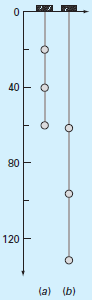
\includegraphics[width=0.1\linewidth]{fig_8_6}
        \caption{\textsf{Positions of three
        individuals connected
        by bungee cords.
        (a) Unstretched and
        (b) stretched.}}
        \label{fig:fig_8_6}
    \end{figure}

\end{example}

\section{\textbf{CASE STUDY} - CURRENTS AND VOLTAGES IN CIRCUITS}
\label{sec:sec_8_3}

\textbf{Background.} Recall that in Chap. 1 (Table 1.1), we summarized some models and associated conservation laws that figure prominently in engineering. As in Fig. 8.7, each model represents a system of interacting elements. Consequently, steady-state balances derived from the conservation laws yield systems of simultaneous equations. In many cases, such systems are linear and hence can be expressed in matrix form. The present case study focuses on one such application: circuit analysis.

A common problem in electrical engineering involves determining the currents and voltages at various locations in resistor circuits. These problems are solved using Kirchhoff's current and voltage rules. The current (or point) rule states that the algebraic sum of all currents entering a node must be zero (Fig. $8.8 a$ ), or

\bigskip
$\sum i=0$ \hfill{(8.8)}
\bigskip

where all current entering the node is considered positive in sign. The current rule is an application of the principle of conservation of charge (recall Table 1.1).

\begin{multicols}{2}

    \begin{figure}[H]
        \centering
        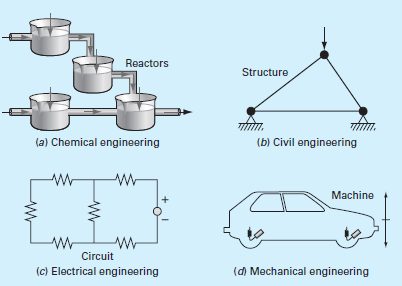
\includegraphics[width=1.1\linewidth]{fig_8_7}
        \caption{\textsf{Engineering systems which, at steady state, can be modeled with linear algebraic
        equations.}}
        \label{fig:fig_8_7}
    \end{figure}
    
    \begin{figure}[H]
        \centering
        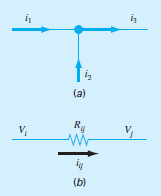
\includegraphics[width=0.65\linewidth]{fig_8_8}
        \caption{\textsf{Schematic representations
        of (a) Kirchhoff's current rule
        and (b) Ohm's law.}}
        \label{fig:fig_8_8}
    \end{figure}
    
\end{multicols}

\noindent The voltage (or loop) rule specifies that the algebraic sum of the potential differences (i.e., voltage changes) in any loop must equal zero. For a resistor circuit, this is expressed as

\bigskip
$\sum \xi-\sum i R=0$ \hfill{(8.9)}
\bigskip

where $\xi$ is the emf (electromotive force) of the voltage sources, and $R$ is the resistance of any resistors on the loop. Note that the second term derives from Ohm's law (Fig. $8.8 \mathrm{~b}$ ), which states that the voltage drop across an ideal resistor is equal to the product of the current and the resistance. Kirchhoff's voltage rule is an expression of the conservation of energy.

\noindent\textbf{Solution.} Application of these rules results in systems of simultaneous linear algebraic equations because the various loops within a circuit are interconnected. For example, consider the circuit shown in Fig. 8.9. The currents associated with this circuit are unknown both in magnitude and direction. This presents no great difficulty because one simply assumes a direction for each current. If the resultant solution from Kirchhoff's laws is negative, then the assumed direction was incorrect. For example, Fig. $8.10$ shows some assumed currents.

\begin{multicols}{2}

    \begin{figure}[H]
        \centering
        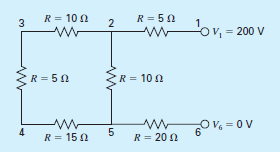
\includegraphics[width=0.7\linewidth]{fig_8_9}
        \caption{\textsf{A resistor circuit to be solved using simultaneous
        linear algebraic equations.}}
        \label{fig:fig_8_9}
    \end{figure}
    
    \begin{figure}[H]
        \centering
        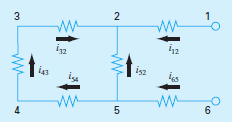
\includegraphics[width=0.7\linewidth]{fig_8_10}
        \caption{\textsf{Assumed current directions.}}
        \label{fig:fig_8_10}
    \end{figure}
    
\end{multicols}

Given these assumptions, Kirchhoff's current rule is applied at each node to yield
$$
\begin{aligned}
&i_{12}+i_{52}+i_{32}=0 \\
&i_{65}-i_{52}-i_{54}=0 \\
&i_{43}-i_{32}=0 \\
&i_{54}-i_{43}=0
\end{aligned}
$$
Application of the voltage rule to each of the two loops gives
$$
\begin{aligned}
&-i_{54} R_{54}-i_{43} R_{43}-i_{32} R_{32}+i_{52} R_{52}=0 \\
&-i_{65} R_{65}-i_{52} R_{52}+i_{12} R_{12}-200=0
\end{aligned}
$$
or, substituting the resistances from Fig. $8.9$ and bringing constants to the right-hand side,
$$
\begin{aligned}
&-15 i_{54}-5 i_{43}-10 i_{32}+10 i_{52}=0 \\
&-20 i_{65}-10 i_{52}+5 i_{12}=200
\end{aligned}
$$
Therefore, the problem amounts to solving six equations with six unknown currents. These equations can be expressed in matrix form as
$$
\left[\begin{array}{cccccc}
1 & 1 & 1 & 0 & 0 & 0 \\
0 & -1 & 0 & 1 & -1 & 0 \\
0 & 0 & -1 & 0 & 0 & 1 \\
0 & 0 & 0 & 0 & 1 & -1 \\
0 & 10 & -10 & 0 & -15 & -5 \\
5 & -10 & 0 & -20 & 0 & 0
\end{array}\right]\left\{\begin{array}{l}
i_{12} \\
i_{52} \\
i_{32} \\
i_{65} \\
i_{54} \\
i_{43}
\end{array}\right\}=\left\{\begin{array}{c}
0 \\
0 \\
0 \\
0 \\
0 \\
200
\end{array}\right\}
$$

Although impractical to solve by hand, this system is easily handled by MATLAB. The solution is

\begin{lstlisting}[numbers=none,frame=none]
    >> A=[1 1 1 0 0 0
    0 -1 0 1 -1 0
    0 0 -1 0 0 1
    0 0 0 0 1 -1
    0 10 -10 0 -15 -5
    5 -10 0 -20 0 0];
    >> b=[0 0 0 0 0 200]';
    >> current=A\b
    current =
        6.1538
        -4.6154
        -1.5385
        -6.1538
        -1.5385
        -1.5385
\end{lstlisting}

Thus, with proper interpretation of the signs of the result, the circuit currents and voltages are as shown in Fig. 8.11. The advantages of using MATLAB for problems of this type should be evident.

\begin{figure}[H]
    \centering
    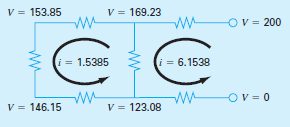
\includegraphics[width=0.5\linewidth]{fig_8_11}
    \caption{\textsf{The solution for currents and voltages obtained using MATLAB.}}
    \label{fig:fig_8_11}
\end{figure}
\newpage

\noindent\textbf{PROBLEMS}

\begin{multicols}{2}
    \noindent \textbf{8.1} Given a square matrix [A], write a single line MATLAB command that will create a new matrix $\left[A u_{g}\right]$ that consists of the original matrix $[A]$ augmented by an identity matrix $[I]$.
    
    \noindent \textbf{8.2} A number of matrices are defined as
    $$
    \begin{aligned}
    &{[A]=\left[\begin{array}{ll}
    4 & 5 \\
    1 & 2 \\
    5 & 6
    \end{array}\right] \quad[B]=\left[\begin{array}{lll}
    4 & 3 & 7 \\
    1 & 2 & 6 \\
    2 & 0 & 4
    \end{array}\right]} \\
    &\{C\}=\left\{\begin{array}{l}
    2 \\
    6 \\
    1
    \end{array}\right\} \quad[D]=\left[\begin{array}{cccc}
    5 & 4 & 3 & -7 \\
    2 & 1 & 7 & 5
    \end{array}\right] \\
    &{[E]=\left[\begin{array}{lll}
    1 & 5 & 6 \\
    7 & 1 & 3 \\
    4 & 0 & 6
    \end{array}\right]} \\
    &{[F]=\left[\begin{array}{lll}
    2 & 0 & 1 \\
    1 & 7 & 4
    \end{array}\right] \quad\lfloor G\rfloor=\left\lfloor\begin{array}{lll}
    8 & 6 & 4
    \end{array}\right]}
    \end{aligned}
    $$
    Answer the following questions regarding these matrices:

    \noindent (a) What are the dimensions of the matrices?

    \noindent (b) Identify the square, column, and row matrices.

    \noindent (c) What are the values of the elements: $a_{12}, b_{23}, d_{32}, e_{22}$, $f_{12}, g_{12} ?$
    
    \noindent (d) Perform the following operations:

    \noindent (1) $[E]+[B]$

    \noindent (2) $[A]+[F]$

    \noindent (3) $[B]-[E]$

    \noindent (4) $7 \times[B]$

    \noindent (5) $\{C\}^{T}$

    \noindent (6) $[E] \times[B]$

    \noindent (7) $[B] \times[E]$

    \noindent (8) $[D]^{T}$
    
    \noindent (9) $[G] \times\{C\}$
    
    \noindent $(10)[I] \times[B]$
    
    \noindent (11) $[E]^{T} \times[E]$
    
    \noindent (12) $\{C\}^{T} \times\{C\}$
    
    \noindent \textbf{8.3} Write the following set of equations in matrix form:
    $$
    \begin{aligned}
    &50=5 x_{3}-6 x_{2} \\
    &2 x_{2}+7 x_{3}+30=0 \\
    &x_{1}-7 x_{3}=50-3 x_{2}+5 x_{1}
    \end{aligned}
    $$
    Use MATLAB to solve for the unknowns. In addition, use it to compute the transpose and the inverse of the coefficient matrix.
    
    \noindent \textbf{8.4} Three matrices are defined as

    \noindent $[A]=\left[\begin{array}{cc}6 & -1 \\ 12 & 7 \\ -5 & 3\end{array}\right][B]=\left[\begin{array}{cc}4 & 0 \\ 0.6 & 8\end{array}\right][C]=\left[\begin{array}{cc}1 & -2 \\ -6 & 1\end{array}\right]$
    
    \noindent (a) Perform all possible multiplications that can be computed between pairs of these matrices.
    
    \noindent (b) Justify why the remaining pairs cannot be multiplied.
    
    \noindent (c) Use the results of (a) to illustrate why the order of multiplication is important.
    
    \noindent \textbf{8.5} Solve the following system with MATLAB:
    $$
    \left[\begin{array}{cc}
    3+2 i & 4 \\
    -i & 1
    \end{array}\right]\left\{\begin{array}{l}
    z_{1} \\
    z_{2}
    \end{array}\right\}=\left\{\begin{array}{c}
    2+i \\
    3
    \end{array}\right\}
    $$
    
    \noindent \textbf{8.6} Develop, debug, and test your own M-file to multiply two matrices that is, $[X]=[Y][Z]$, where $[Y]$ is $m$ by $n$ and $[Z]$ is $n$ by $p$. Employ \texttt{for... end} loops to implement the multiplication and include error traps to flag bad cases. Test the program using the matrices from Prob. 8.4.
    
    \noindent \textbf{8.7} Develop, debug, and test your own M-file to generate the transpose of a matrix. Employ \texttt{for... end} loops to implement the transpose. Test it on the matrices from Prob. 8.4.
    
    \noindent \textbf{8.8} Develop, debug, and test your own M-file function to switch the rows of a matrix using a permutation matrix. The first lines of the function should be as follows:
    
    \begin{lstlisting}[numbers=none,frame=none]
    function B = permut(A,r1,r2)
    % Permut: Switch rows of matrix A
    % with a permutation matrix
    % B = permut(A,r1,r2)
    % input:
    % A = original matrix
    % r1, r2 = rows to be switched
    % output:
    % B = matrix with rows switched
	\end{lstlisting}

    Include error traps for erroneous inputs (e.g., user specifies rows that exceed the dimensions of the original matrix).
    
    \noindent \textbf{8.9} Five reactors linked by pipes are shown in Fig. P8.9. The rate of mass flow through each pipe is computed as the product of flow $(Q)$ and concentration $(c)$. At steady state, the mass flow into and out of each reactor must be equal. For example, for the first reactor, a mass balance can be written as
    $$
    Q_{01} c_{01}+Q_{31} c_{3}=Q_{15} c_{1}+Q_{12} c_{1}
    $$
    Write mass balances for the remaining reactors in Fig. P8.9 and express the equations in matrix form. Then use MATLAB to solve for the concentrations in each reactor.
    
    \begin{figure}[H]
        \centering
        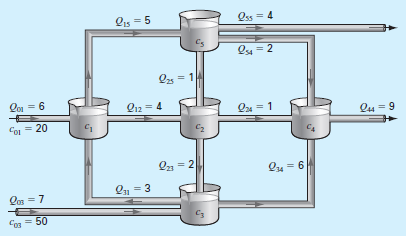
\includegraphics[width=1\linewidth]{fig_P8_9}
        \caption{\textsf{FIGURE P8.9}}
        \label{fig:fig_P8_9}
    \end{figure}

    \noindent \textbf{8.10} An important problem in structural engineering is that of finding the forces in a statically detemminate truss (Fig. P8.10). This type of structure can be described as a system of coupled linear algebraic equations derived from force balances. The sum of the forces in both horizontal and
    vertical directions must be zero at each node, because the system is at rest. Therefore, for node 1:
    $$
    \begin{aligned}
    &\sum F_{H}=0=-F_{1} \cos 30^{\circ}+F_{3} \cos 60^{\circ}+F_{1, h} \\
    &\sum F_{V}=0=-F_{1} \sin 30^{\circ}-F_{3} \sin 60^{\circ}+F_{1, v}
    \end{aligned}
    $$
    for node 2:
    $$
    \begin{aligned}
    &\sum F_{H}=0=F_{2}+F_{1} \cos 30^{\circ}+F_{2, h}+H_{2} \\
    &\sum F_{V}=0=F_{1} \sin 30^{\circ}+F_{2, v}+V_{2}
    \end{aligned}
    $$
    for node 3 :
    $$
    \begin{aligned}
    &\sum F_{H}=0=-F_{2}-F_{3} \cos 60^{\circ}+F_{3, h} \\
    &\sum F_{V}=0=F_{3} \sin 60^{\circ}+F_{3, \vee}+V_{3}
    \end{aligned}
    $$
    where $F_{i, h}$ is the external horizontal force applied to node $i$ (where a positive force is from left to right) and $F_{i, v}$ is the external vertical force applied to node $i$ (where a positive force is upward). Thus, in this problem, the $2000-\mathrm{N}$ downward force on node 1 corresponds to $F_{i, v}=-2000$. For this case, all other $F_{i, b}$ 's and $F_{i \lambda h}$ 's are zero. Express this set of linear algebraic equations in matrix form and then use MATLAB to solve for the unknowns.

    \begin{figure}[H]
        \centering
        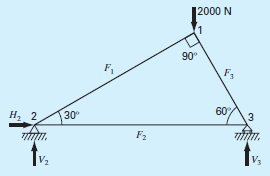
\includegraphics[width=1\linewidth]{fig_P8_10}
        \caption{\textsf{FIGURE P8.10}}
        \label{fig:fig_P8_10}
    \end{figure}

    \noindent \textbf{8.11} Consider the three mass-four spring system in Fig. P8.11. Determining the equations of motion from $\Sigma F_{x}=$ $m a_{x}$ for each mass using its free-body diagram results in the
    following differential equations:
    $$
    \begin{aligned}
    &\vec{x}_{1}+\left(\frac{k_{1}+k_{2}}{m_{1}}\right) x_{1}-\left(\frac{k_{2}}{m_{1}}\right) x_{2}=0 \\
    &\vec{x}_{2}-\left(\frac{k_{2}}{m_{2}}\right) x_{1}+\left(\frac{k_{2}+k_{3}}{m_{2}}\right) x_{2}-\left(\frac{k_{3}}{m_{2}}\right) x_{3}=0 \\
    &\vec{x}_{3}-\left(\frac{k_{3}}{m_{3}}\right) x_{2}+\left(\frac{k_{3}+k_{4}}{m_{3}}\right) x_{3}=0
    \end{aligned}
    $$
    where $k_{1}=k_{4}=10 \mathrm{~N} / \mathrm{m}, k_{2}=k_{3}=40 \mathrm{~N} / \mathrm{m}$, and $m_{1}=m_{2}=$ $m_{3}=1 \mathrm{~kg}$. The three equations can be written in matrix form:
    $0=\{$ Acceleration vector $\}$
    $+[k / m$ matrix $]$ displacement vector $x\}$
    At a specific time where $x_{1}=0.05 \mathrm{~m}, x_{2}=0.04 \mathrm{~m}$, and $x_{3}=$ $0.03 \mathrm{~m}$, this forms a tridiagonal matrix. Use MATLAB to solve for the acceleration of each mass.
    
    \begin{figure}[H]
        \centering
        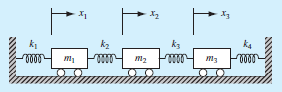
\includegraphics[width=1\linewidth]{fig_P8_11}
        \caption{\textsf{FIGURE P8.11}}
        \label{fig:fig_P8_11}
    \end{figure}

    \noindent \textbf{8.12} Perfom the same computation as in Example 8.2, but use five jumpers with the following characteristics:
    \begin{tabular}{cccc} 
    Jumper & Mass $(\mathbf{k g})$ & Spring  & Unstretched \\
    & & Constant $(\mathbf{N} / \mathbf{m})$ & Cord Length $(\mathbf{m})$ \\
    \hline 1 & 65 & 80 & 10 \\
    2 & 75 & 40 & 10 \\
    3 & 60 & 70 & 10 \\
    4 & 75 & 100 & 10 \\
    5 & 90 & 20 & 10
    \end{tabular}

    \noindent \textbf{8.13} Three masses are suspended vertically by a series of identical springs where mass 1 is at the top and mass 3 is at the bottom. If $\mathrm{g}=9.81 \mathrm{~m} / \mathrm{s}^{2}, m_{1}=2 \mathrm{~kg}, m_{2}=2.5 \mathrm{~kg}, m_{3}=$ $3 \mathrm{~kg}$, and the $k^{\prime} \mathrm{s}=15 \mathrm{~kg} / \mathrm{s}^{2}$, use MATLAB to solve for the displacements $x$.
    
    \noindent \textbf{8.14} Perform the same computation as in Sec. 8.3, but for the circuit in Fig. P8.14.
    
    \begin{figure}[H]
        \centering
        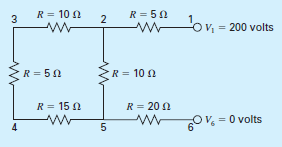
\includegraphics[width=1\linewidth]{fig_P8_14}
        \caption{\textsf{FIGURE P8.14}}
        \label{fig:fig_P8_14}
    \end{figure}

    \noindent \textbf{8.15} Perform the same computation as in Sec. 8.3, but for the circuit in Fig. P8.15.

    \begin{figure}[H]
        \centering
        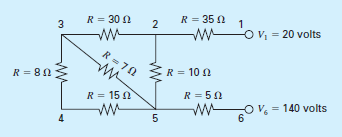
\includegraphics[width=1\linewidth]{fig_P8_15}
        \caption{\textsf{FIGURE P8.15}}
        \label{fig:fig_P8_15}
    \end{figure}

\end{multicols}

\end{document}